%Florian Bogner & Alexander Palmrich

\documentclass[a4paper,12pt]{paper}
\usepackage{fullpage}
\usepackage[utf8]{inputenc}
%\usepackage[ngerman]{babel}
\usepackage[english]{babel}
\usepackage{amsmath}
\usepackage{amssymb}
\usepackage{latexsym}
\usepackage{mathtools}
\usepackage{listings}
%\usepackage{algorithm}
%\usepackage{algpseudocode}
\usepackage{graphicx}
\usepackage{booktabs}
\usepackage{hhline}
\usepackage{amsthm}
\usepackage{cite}

\theoremstyle{plain}
\newtheorem{thm}{Theorem}[section] % reset theorem numbering for each chapter

\theoremstyle{definition}
\newtheorem{defn}[thm]{Definition} % definition numbers are dependent on theorem numbers
\newtheorem{exmp}[thm]{Example} % same for example numbers
\newtheorem{lem}[thm]{Lemma}
%https://tex.stackexchange.com/questions/45817/theorem-definition-lemma-problem-numbering


\begin{document}

\begin{titlepage}
\huge
\centering
Border Propagation: A Novel Approach To Determining Slope Region Decompositions

\vfill

\normalsize
Florian Bogner \& Alexander Palmrich
\end{titlepage}




\tableofcontents
\newpage

%% high level abstract: %%
% - motivate slope region with 2D function surface
% - define slope region for any dimension
% - reference known algorithm
% - motivate new algorithm for continuous case
% - describe discrete algorithm
% - many many fancy pictures

\section{Abstract}

TODO
mention slope regions as defined in here\cite{kropatsch2019space}

\section{Motivating Slope Regions}

In this section we try to develop an intuitive understanding of the term \emph{slope region} and its generalization to dimensions higher than 2. The concise definitions of the terms already employed here is reserved for the next section.

Consider an image, either gray-scale or in color. If it is a color image, it can be decomposed into its color channels, which can individually be read as gray-scale images. We now think of the light intensity (i.e. the image value) of one such gray-scale image as the height of a landscape, yielding a surface in 3D space. The surface will have hills in areas where the image is bright, and will have dales in dark areas. Please refer to figure \ref{fig:conversion} for a visualization!


\begin{figure}[h]
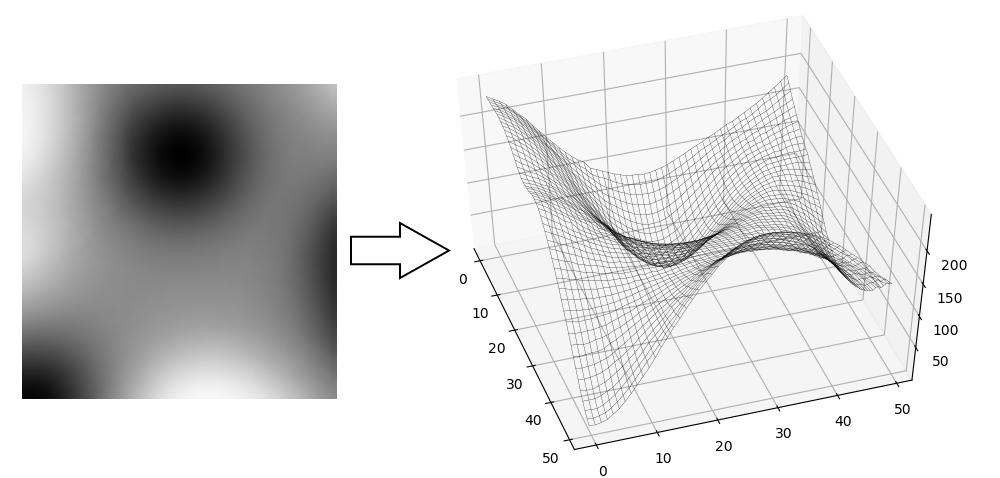
\includegraphics[width=\textwidth]{img/visu1.png}
\caption{Gray-scale to Height-map conversion}
\label{fig:conversion}
\end{figure}

Our aim now is to partition the surface into \emph{regions} (i.e. subsets) in a particular way: We require each region to consist only of a single slope, by which we mean that we can ascend (or descend) from any given point of the region, to any other given point of the region, along a path that runs entirely within the region. Such a decomposition is not unique, but we can at least try to get a partition \emph{as coarse as possible}, meaning that we merge slope regions if the resulting subset is still a slope region, and we iterate this until it can be done no more. There might be many different such coarsest slope decompositions, but we accept any one of them.

The criterion we used to describe slopes, any two points being connected by either an ascending or a descending path, can easily be used in higher dimensions. Think of a computer tomography scan, which will yield gray-scale data, but not just as a 2D image, but rather on a 3D volume.
Now, if you are inclined to visualize a fourth spacial dimension, you can think of that fourth direction as the height of a 3D hyper-surface in 4D space, with the height encoded in the tomography scan. But imagining this is difficult and not required, because our slope region criterion works just fine here: We want to partition the 3D volume, such that any two points in a region can be connected via an either ascending or descending path within the region. Recall that \emph{ascending} and \emph{descending} refers to the brightness value of the tomography scan as we move in the volume.

By abstracting from image and tomography to a real function defined on some subset of $\mathbb{R}^n$ (think of it as the brightness function!), and by rigorously defining a coarsest slope decomposition, we can lift the concept to arbitrary dimensions in a mathematically concise fashion.

\section{Definitions}

In this and the following chapters we will consider a set $\Omega \subset \mathbb{R}^n$ with $n > 1$ and a continuous function $f: \Omega \mapsto \mathbb{R}$.

\begin{defn}
A path $\gamma: [a,b] \to \Omega$ is called \emph{monotonic} if and only if it is continuous and
\begin{align*}
\forall & s, t \in [a,b]: s < t \Rightarrow f(\gamma(s)) \leq f(\gamma(t)) ~ \lor \\
\forall & s, t \in [a,b]: s < t \Rightarrow f(\gamma(s)) \geq f(\gamma(t))
\end{align*}
\end{defn}

\begin{defn}
Let $R \subset \Omega$. $R$ is called \emph{slope region} or \emph{monotonically connected} if and only if for all $x, y \in R$ there exists a monotonic path $\gamma: [a,b] \to R$ with $\gamma(a) = x$ and $\gamma(b) = y$.
\end{defn}

\begin{defn}
A family of sets $\left\{ A_i \subset \Omega \mid i \in I \right\}$ is called a \emph{slope region decomposition} if and only if:
\begin{itemize}
\item $A_i$ is a slope region for all $i \in I$
\item $\forall i,j \in I: i \neq j \Rightarrow A_i \cap A_j = \emptyset$.
\item $\bigcup_{i\in I} A_i = \Omega$
\end{itemize}
\end{defn}

%\begin{defn}
%A slope region decomposition $\left\{ R_i \subset \Omega \mid i \in I \right\}$ is called \emph{maximally coarse} or simply \emph{coarse} if and only if there is no $J \subset I$ with $|J| \geq 2$ and
%\begin{equation*}
%\left\{ R_i \subset \Omega \mid i \in I \setminus J \right\} \cup \left\{ \bigcup_{j\in J} R_j \right\}
%\end{equation*}
%\end{defn}


\begin{defn}
Consider two slope region decompositions $\mathcal{A} = \left\{ A_i \subset \Omega \mid i \in I \right\}$ and $\mathcal{B} = \left\{ B_j \subset \Omega \mid j \in J \right\}$. We call $\mathcal{A}$ \emph{coarser than} $\mathcal{B}$, in Symbols $\mathcal{A} \succeq \mathcal{B}$ if and only if
\begin{equation*}
\forall j \in J ~ \exists i \in I: B_j \subset A_i.
\end{equation*}
\end{defn}

\begin{lem}
$\succeq$ is a partial order, i.e. fulfills reflexivity, antisymmetry and transitivity.

\emph{Proof:} trivial \hfill $\Box$
\end{lem}

\begin{defn}
A slope region decomposition $\mathcal{A}$ is called \emph{maximally coarse} or simply \emph{coarse} if and only if there is no other coarser slope region decomposition.
\end{defn}

\begin{lem}
Let $A \subset \Omega$ be a path-connected set. $A$ is a slope region if and only if all levelsets of $f$ in $A$ are path-connected, i.e.
\begin{equation*}
\forall c \in \mathbb{R}: f^{-1}(c) \cap A ~ \text{is path-connected}.
\end{equation*}
\end{lem}

\emph{Proof:} "$\Rightarrow$" via contraposition:

Suppose there exists a $c \in \mathbb{R}$ with $L := f^{-1}(c) \cap A$ not path-connected. We decompose $L$ in its components and pick $x$ and $y$ from different components. Since $f(x) = f(y) = c$ a monotonic path between $x$ and $y$ would have to lie completely in L. However, since $x$ and $y$ are from different components, they cannot be connected by a path in $L$ and therefore cannot be connected with a monotonic path. Therefore, A is not a slope region.

$~$

\begin{wrapfigure}{r}{0.4\textwidth}
\centering
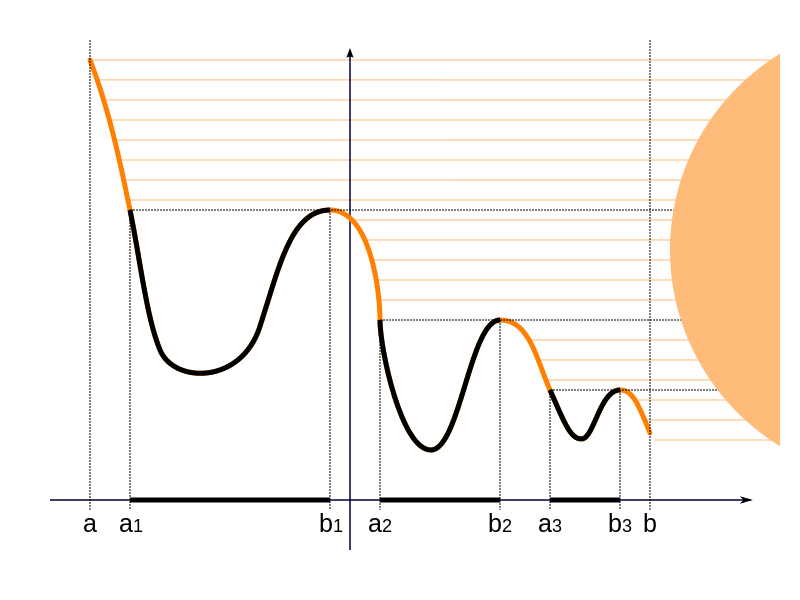
\includegraphics[width=0.4\textwidth]{img/Rising_sun_lemma.png}
\caption{Rising sun lemma}
\label{fig:lemma_1}
\end{wrapfigure}

"$\Leftarrow$" via \emph{ironing out} an arbitrary path:

Given $x, y \in A$ we have to find a monotonic path $\gamma$. Without loss of generality suppose $f(x) \geq f(y)$. Since $A$ is path-connected, there exists an (not necessarily monotonic) path $\gamma_0: [a,b] \to A$ from $x$ to $y$. Using the Rising Sun lemma \cite{grill} on the continuous function $f \circ \gamma_0$ we get the \emph{shadow} $S = \bigcup_{i \in I} (a_n, b_n)$ consisting of at most countably many intervals.

$S$ consists of the points which contradict the monotony of $f \circ \gamma_0$, thus we want to \emph{iron out} these points.

Let $c_n := f(a_n) = f(b_n)$. Since the levelset of $c_n$ is path-connected, we can connect $\gamma_0(a_n)$ and $\gamma_0(b_n)$ with a level path $\gamma_n^* : [a_n, b_n] \to A.$

Finally, we define:
\begin{equation*}
\gamma(\sigma) :=
\begin{cases}
\gamma_n^*(\sigma) & \sigma \in [a_n, b_n] \\
\gamma_0(\sigma) & \text{elsewhere}
\end{cases}
\end{equation*}

$\gamma$ is a monotonic path from $x$ to $y$, thus $A$ is a slope region.

\hfill $\Box$



\section{Motivating The Border Propagation Algorithm}
We will now work our way to the central insights on which the border propagation algorithm hinges.

Slope regions can be constructed and grown in a straight-forward iterative manner by sweeping through the function values from lowest to highest. This is similar to the intuition employed in Morse theory\cite{MatsumotoYukio2002AitM}. Visualize a smooth, compact 2D surface in 3D space. Initially, our decomposition is empty, i.e. there are no slope regions (and we thus don't yet have an actual \emph{decomposition}).

Starting at the global minimum, we add a new region, containing only the argmin (i.e. a single point on the 2D image where the minimal value is taken). Imagine a water level rising from below the surface, up to the point of first contact. Now, there might be many points where the global minimum is taken. This will either be due to flat regions (\emph{plateaus}) on the surface, which we want to include into the single existing region, or it will be due to individual dales, which all have their lowest point at the same height.

In this second case, we can't put the points into the existing region, because we would not be able to get from one argmin to another via a monotonic path. Instead, we need to add a new region for each individual dale, that is to say we need to look at the connected components of the levelset and assign to each component a new region.

As the water rises, we can add points to an existing region growing it upwards if they are just outside the region\footnote{Why can we do that? By adding only points which are connected to the region we ensure path-connectedness, and by growing the region upwards, we can construct ascending paths from old points to new ones. The smoothness of the surface guarantees that while moving at a fixed height, we can reach all points of the region with that height.}. Otherwise they correspond to a distant local minimum and have to be dealt with as before, by opening a new region for each point (or rather, each connected component).

With the water rising further still, the regions will grow upwards to a point where they meet. Any such point is a saddle point, and we have to account for it the next time we want to grow any one of the touching regions. The saddle point connects the edges of the regions which meet in it, at the current height of the water level. It might be the case that the not-yet-assigned points (the ones above the water) get separated into multiple connected components, or they might remain connected.

If the points remain connected, then we have to decide for a single one of the involved regions to be allowed to grow upwards from the component. This means that one region effectively inherits the growth directions from the other region(s). The other region(s) lose their potential for expansion and remain frozen in their current state.

If the unassigned points have multiple components, then we may assign one component to each involved region. The regions will then grow only in the directions determined by the assigned components as the water rises. Any region without assigned component remains frozen. Should there be more components than regions, then we open up a new region for each surplus component.

An oddity which can occur are self-loops: A region might grow into a "C"-shape, and then proceed to close up into an "O"-shape. This case can be treated similarly as above, the only difference is that the saddle is found by recognizing that the region collides with itself, instead of with another region.

Eventually this procedure will arrive at the global maximum, and the entire surface will be divided into regions. Since we proceeded with the necessary care and attention along the way, we ensured that the regions remained slope regions, and we also only created additional regions when we absolutely had to, showing that the resulting composition is maximally coarse.

The same algorithm can be applied in higher dimensions. We deal with iso-hyper-surfaces as level sets, but the topological considerations about connectedness remain the same as in the illustrative 2D case.


\bibliography{lit}
\bibliographystyle{plain}
\end{document}
































